\documentclass[12pt]{article}

\usepackage{booktabs}
\usepackage[dvipsnames]{xcolor}
\usepackage{minted}
\usepackage{sbc-template}
\usepackage{graphicx,url}
\usepackage[utf8]{inputenc}
\usepackage[portuguese]{babel}

\sloppy

\title{Previsão de resultados de partidas profissionais de \\ \textit{Counter Strike - Global Offensive}}

\author{Leonardo Ribeiro Santiago (120036072)\inst{1} }


\address{Instituto de Computação -- Universidade Federal do Rio de Janeiro
  (UFRJ) \\
  Av. Pedro Calmon, 550 –- Cidade Universitária da Universidade Federal do Rio de Janeiro \\ Rio de Janeiro -– RJ -- 21941-901}

\begin{document} 

\maketitle

\begin{resumo}
  Neste trabalho, utilizamos dados de partidas profissionais do jogo \textit{Counter Strike - Global Offensive} para treinar modelos de predição do resultado de partidas futuras. Para isso, aplicamos técnicas de pre-processamento a um dataset de informações obtidas do site \url{https://www.hltv.org} (através de \textit{web scrapping}) para analisar médias históricas de estatísticas relevantes de cada jogador de uma partida. Com esses dados, determinamos quais estatísticas são mais relevantes para a classificação de resultados usando técnicas de modelagem.
\end{resumo}

\section{Introdução}

Counter Strike Global Offensive é um jogo de tiro em primeira pessoa mais populares e influentes de toda a história, onde dezenas de partidas valendo centenas de milhares de dólares são disputadas por times profissionais ao redor do mundo. O jogo fora lançado em agosto de 2012, quarto na série \textit{Counter Strike}, lançado como um sucessor do \textit{Counter Strike - Source}. Em 2023, o jogo fora atualizado para uma nova versão, chamada de Counter Strike 2, trazendo várias mudanças estéticas e de balanceamento geral, mas mantendo os elementos principais da jogabilidade. Entretanto, por ser muito recente (menos de 1 ano), os dados disponíveis de partidas profissionais de \textit{Counter Strike 2} são escassos, e portanto utilizaremos um dataset de partidas de \textit{Counter Strike - Global Offensive} no período de 2015-2020.

Em cada partida de CSGO, os 2 lados - terroristas e contra-terroristas - compostos por 5 jogadores batalham para ganhar 16 rounds em um mapa. Para ganhar um round, os terroristas devem matar o time inimigo inteiro ou plantar a bomba (chamada de C4) antes que o tempo do round (1 minuto e 55 segundos) acabe. Em contra partida, os contra-terroristas ganham se o tempo acabar sem que os terroristas plantem a bomba ou se matarem o time inimigo inteiro. Se a bomba for plantada, os contra-terroristas tem 40 segundos para defusar a bomba (independente do tempo restante do round), enquanto os terroristas devem impedir que defusem a bomba.

Após os 15 primeiros rounds, os times invertem de lado e reinicia-se a economia para o estado inicial, independente do resultado da primeira metade da partida. Caso haja empate 15-15, a economia é resetada para um valor fixo, e os times competem uma prorrogação para ganhar 4 dos próximos 6 rounds. Se ocorrer empate na prorrogação, é iniciada outra prorrogação da mesma forma, ad infinitum, até que haja um ganhador no mapa.

Grande parte da estratégia do jogo advém de sua economia interna: cada jogador tem seu próprio dinheiro para comprar armas,quipamentos e granadas para o round, que serão carregados para o round seguinte caso sobreviva, obtendo dinheiro através de ações chaves como matar inimigos e plantar a bomba, além de um valor fixo por cada round - e obviamente recebe-se muito mais quando o round é ganho. Ambos os times começam com a exata mesma quantia de dinheiro, e a economia de rounds futuros é determinada inteiramente pelo resultado de rounds passados.

É importante ressaltar que a todo momento existem 7 mapas que podem ser jogados em competições, e mudanças a esses mapas ocasionalmente ocorrem (geralmente, retira-se um mapa e adiciona-se um novo por ano). Geralmente partidas profissionais são jogadas no formato melhor de 3, mas o dataset escolhido é composto apenas de partidas melhores de 1 e de 3. Para decidir o mapa jogado no caso de melhor de 1, os times alternam para remover mapas, começando pelo ``Time 1'', deixando o ``Time 2'' decidir qual mapa será jogado, resultando no ``Time 1'' escolhendo o lado que irá começar no mapa (terrorista ou contra-terrorista). No caso de melhor de 3, os times alternam para remover um mapa cada, depois alternam para escolher um mapa a ser jogado, e por fim alternam para remover um mapa, sendo escolhido o como terceiro o mapa restante.

O objetivo deste trabalho é, portanto, utilizar estatísticas dos jogadores em \textbf{partidas passadas} para prever resultados de partidas não vistas ainda. Para isso, montaremos um sistema para calcular a influência de resultados passados de um jogador específico em relação ao tempo, processar os dados de forma a descobrir as estatísticas exatas para cada jogador em relação as partidas prévias disponíveis no dataset, e finalmente treinar modelos de classificação em cima desses dados para prever o resultado da partida, sem utilizar nenhum dado do resultado da partida.

\section{Dataset}

O dataset escolhido (\cite{dataset}) é composto de 4 arquivos:

\subsection{picks.csv}

Contém informações da sequência de \textit{picks} e \textit{bans} para cada partida, especificando quais mapas foram banidos e escolhidos por cada time, em qual ordem, e se a partida é melhor de 1 ou melhor de 3.

\subsection{economy.csv}

Para cada partida listada, contém a quantidade de dinheiro total de cada time em cada round nos primeiros 30 rounds de um mapa, junto com o ganhador de cada round.

\subsection{results.csv}

Para cada partida listada, contém o nome dos times, o mapa jogado, se é melhor de 1 ou melhor de 3, e o resultado de cada mapa.

\subsection{players.csv}

Para cada partida listada, contém a informação do nome e id do jogador, relacionando com a partida jogada. Além disso, fornece por jogador estatísticas disponíveis no site da HLTV:
\begin{itemize}
\item \textbf{Abates}: quantos inimigos o jogador abateu
\item \textbf{Mortes}: quantas vezes o jogador morreu
\item \textbf{Assistências}: quantas assistências um jogador conseguiu - geralmente configura-se assistência quando um jogador dá mais de 40\% da vida em dano em um inimigo, e outro jogador do time abate esse inimigo.
\item \textbf{Número de abates por tiro na cabeça}: número de abates que o jogador conseguiu onde o último tiro foi na cabeça. No jogo, tiros na cabeça dão 4 vezes mais dano, logo jogadores com taxas maiores de tiros na cabeça tendem a matar mais.
\item \textbf{Número de assistências por flashbang}: a granada flashbang cega jogadores que olham para ela (tornando a tela dos que olham diretamente branca por alguns segundos), e cegar um inimigo conta como uma assistência.
\item \textbf{KAST} (Kill, Assist, Survival, Traded): Estatística gerada pela própria HLTV, significando a porcentagem de rounds em que o jogador pegou uma kill, uma assistência, sobreviveu ou foi trocado (um amigo abateu o inimigo que te matou).
\item \textbf{Dano médio por round (ADR)}: Quantidade total de dano dado no jogo dividido pela quantidade de rounds do mapa.
\item \textbf{Diferença de abates e mortes}: Diferença entre o número de abates e o número de mortes.
\item \textbf{Diferença de primeiros abates}: Diferença entre o número de vezes em que o jogador foi o primeiro a morrer no round e o número de vezes em que o jogador foi o primeiro a matar no round.
\item \textbf{HLTV Rating}: Estatística gerada pela própria HLTV, sendo uma pontuação geral para a performance de um jogador na partida. A fórmula exata para essa estatística não é divulgada publicamente, mas ela utiliza os dados mencionados previamente, bem como outros dados para gerar um número atrelado diretamente ao quão bem um jogador foi na partida.
\end{itemize}

Em cada linha, para cada jogador de uma partida temos essas 10 estatísticas para o primeiro, segundo, e terceiro mapa, bem como para os lados terrorista e contra-terrorista separadamente para cada um dos mapas. Algumas entradas podem estar vazias, a depender se a partida é melhor de 1, ou se o resultado da melhor de 3 for 2 a 0, que acarreta em o terceiro mapa não ser jogado.

\section{Trabalhos relacionados}

O dataset possui 12 estudos relacionados no Kaggle. Dentre eles, vale destacar:
\begin{itemize}
\item \textbf{Rating and Predicting (e)Sports With Jax} \cite{jaxElo}: um modelo de redes neural é montado para assinalar uma pontuação ELO para cada time, e esse modelo é aplicado a vários esportes, incluindo este dataset de Counter Strike. Diferentemente do nosso, o modelo utiliza apenas os resultados de cada partida (sem estatísticas de jogadores) para prever a força dos times em ELO.
\item \textbf{CS:GO Navi Win/Loss Predicting} \cite{navi}: um modelo de redes neurais que utiliza \textit{XGBoosting} é montado em menor escala, para tentar prever o resultado de uma partida entre dois times de counter strike. Igualmente ao anterior, ele apenas observa os resultados de jogos, sem utilizar nenhuma estatística. \url{}
\item \textbf{CS:GO - Was Astralis cheating all along?} \cite{astralis}: Uma análise detalhada sobre as taxas de vitórias e estatísticas do time mais dominante dos anos 2018 e 2019 (ganhando quase todos os torneios importantes desses 2 anos) tentando determinar se existe a possibilidade de estarem usando de meios ilegais para ganhar - concluindo que não.
\item \textbf{Glicko2 Prediction} \cite{glicko2}: Previsão de resultados de jogos, mas ao invés de utilizar médias históricas, é utilizado um algoritmo para decidir o \textit{Glicko2 Rating} (um sistema parecido com ELO) de cada jogador, e utiliza isso para prever jogos, atingindo acurácias de 55\% a 60\%. Esse estudo é mais parecido com o que queremos fazer, em que ele não utiliza dados atrelados a partida para prever o ganhador da partida.
\end{itemize}

\section{Metodologia e pre-processamento}

Para treinar o modelo, iremos considerar as estatísticas passadas - listadas no \textbf{players.csv} - de cada jogador em dada partida. Temos uma assunção principal, que irá motivar a equação, que é a ideia de que performances mais recentes irão correlacionar mais com a performance atual de um jogador do que performances antigas. Assim, utilizaremos a seguinte equação para calcular a média histórica de cada estatística $S$ de um jogador:
\begin{equation}
  S(t) = \sum_{partida}^{T_{partida} > t} \frac{ S_{partida}}{e^{\sqrt{T_{partida} - t}}}
\end{equation}

Na equação, $S_{partida}$ e $T_{partida}$ representam respectivamente o valor da estatística $S$ e a data na partida de index $partida$, e $t$ representa o tempo atual.

Isto é, para dada estatística $S$ de um jogador, calculamos a média histórica dela como a soma dessa estatística para todas as partidas ($S_{partida}$) que ocorreram antes, escalando cada termo dependendo de quão distante no tempo foi tal partida. Fazemos isso para darmos mais importância a performances mais recentes nos dados, de forma a gerar um viés para resultados mais próximos temporalmente. É importante notar que consideramos apenas partidas que vieram \textbf{antes} do tempo atual $t$.

Infelizmente, o ganhador da partida não é listado no \textbf{players.csv}, apenas no \textbf{results.csv}. Portanto, apesar de termos 383.318 entradas no \textbf{players.csv} - ou seja, considerando 10 jogadores por partida, aproximadamente 38.000 partidas - só poderemos usar dessas aquelas que contém um \verb+match_id+ correspondente no \textbf{results.csv}. Ainda sim, temos 45.774 resultados de partidas, mas elas não correspondem um pra um com as listadas no \textbf{players.csv}, e portanto a estratégia utilizada é de iterar por todas as partidas, de forma a acumular todas as partidas válidas, depois acumular todas as estatísticas históricas de cada jogador para cada instância de tempo $t$, junto de quais jogadores estiveram em quais partidas, e por fim gerar o csv final a partir das partidas, procurando a partir de cada partida se temos dados históricos para cada jogador.

Para isso, precisamos lidar tanto no caso de não termos dados sobre algum jogador (não foi incluido no dataset), quanto o caso em que temos dados mas estamos na primeira partida jogada no histórico e não podemos analizar partidas prévias. Por simplicidade, emitimos em ambos os casos o valor \verb+NaN+ em todas as estatísticas. Alguns modelos conseguem utilizar o fato de que não temos informações para todas as colunas para realizar classificações, e portanto incluimos linhas ainda que não tenhamos dados para todos os jogadores, tendo uma única restrição que ao menos 1 dos 10 jogadores tenham informação. Também filtramos casos em que uma partida tenha mais de 10 jogadores já que raramente acontecem (provavelmente um fora substituido no meio do jogo por algum imprevisto) e dificultam a análise.

O algoritmo de preprocessamento pode ser representado como o seguinte pseudo código em python:
\begin{minted}[breaklines, frame=single, fontsize=\footnotesize]{python}
partidas = { partida.match_id: partida for partida in parse('data/results.csv') }
estatisticas_por_jogador = {}
jogadores_em_partida = {}
for jogador in parse('data/players.csv'):
  salvar_dados_historicos(jogos, jogador)
  jogadores_em_partida[jogador.match_id].append(jogador)

with open(output, 'w') as f:
for p in partidas:
  jogadores = jogadores_em_partida.get(p.match_id, [])
  if 0 < len(jogadores) < 10:
     stats = []
     for j in jogadores:
       maybe_stats = estatisticas_por_jogador.get(j.player_id, None)
       stats.append(maybe_stats.get(partida.date) if maybe_stats is not None else ALL_NANS)
     f.write(stats)
\end{minted}

Para realizar esse preprocessamento de forma rápida e correta, foi escrito um programa na linguagem Rust, que compila para um binário executável que, quando executado, processa os dados e salva-os em um arquivo csv, onde cada linha contém as estatísticas históricas de cada jogador do time 1 concatenadas as estatísticas históricas de cada jogador do time 2, para cada partida listada no arquivo \textbf{results.csv}, e o respectivo ganhador da partida (0 para time 1, 1 para time 2). Ao executar, podemos escolher quais estatísticas queremos incluir através de flags de comando ao chamar o programa. Por exemplo, podemos passar \verb+--kill+ \verb+--deaths+ para gerar os dados apenas com informações de abates e mortes por jogador, para podermos experimentar com quais colunas são as mais importantes para obter os melhores resultados.

Para simplificar, não consideraremos relevantes 2 das 10 estatísticas: diferença de abates e mortes, pois está diretamente atrelado as estatísticas de abates e mortes (e portanto um modelo provavelmente conseguiria inferir algo) e número de assistências por flashbangs, dado que nem todas as partidas possuem essa estatística (acredito ser uma estatística mais nova, e por tanto jogos antigos não a possuem).

No total, ao aplicar esse pre-processamento, temos 26.404 partidas com alguma informação de algum jogador, e dessas 4332 possuem ao menos um jogador com valor \verb+NaN+, logo temos 22.072 partidas com todas as informações de todos os jogadores, e podemos escolher quais estatísticas incluir para cada arquivo csv, de forma a facilitar a experimentação. 

\section{Experimentos}

\subsection{Seleção de atributos}

Primeiro, precisamos descobrir quais os atributos mais importantes para treinar os modelos. Para isso, começamos determinando a correlação entre os dados, gerando um arquivo `all-fields.csv` com todos as estatísticas, e concatenamos as informações de cada jogador \textit{row wise} em cada partida, junto se o jogador ganhou ou perdeu. Depois, usamos o pandas para calcular a correlação de cada campo com o campo \verb+Vitória+. O resultado é a seguinte matriz de correlação, ordenada de maior para menor:

\begin{center}
\begin{tabular}{lr}
\toprule
Estatísticas & Vitória \\
\midrule
Vitória & 1.000000 \\
KAST & 0.210676 \\
Rating & 0.200908 \\
ADR & 0.132295 \\
Abates & 0.107173 \\
FKDiff & 0.104344 \\
Assistências & 0.066728 \\
Tiros na Cabeça & 0.062313 \\
Mortes & -0.159766 \\
\bottomrule
\end{tabular}
\end{center}

Surpreendentemente, vemos que \verb+Kast+ é o campo que mais correlaciona com a vitória, logo seguido de Rating, o que é esperado já que o Rating é feito para ser um medidor da performance de um time,.  Vemos que \verb+Tiros na Cabeça+ e \verb+Assistências+ são os menos relacionados, e que a quantidade de mortes é inversamente relacionada com a vitória. Fazendo a mesma análise para as médias das estatísticas de todo o time (ao invés de por jogador), obtemos a seguinte matriz de correlação:

\begin{center}
\begin{tabular}{lr}
\toprule
 & Vitória \\
\midrule
Vitória & 1.000000 \\
Rating & 0.271144 \\
KAST & 0.257011 \\
ADR & 0.254884 \\
FKDiff & 0.203674 \\
Abates & 0.160975 \\
Tiros na Cabeça & 0.124926 \\
Assistências & 0.107955 \\
Mortes & -0.175039 \\
\bottomrule
\end{tabular}
\end{center}

Dessa vez, vemos que a média de Rating de um time de fato é o campo que mais tem relação, logo seguido da média de KAST e da média de ADR. Entretanto, observando a matriz de correlação, podemos ver que Rating tem alta corerlação com esses dois campos:

\begin{center}
  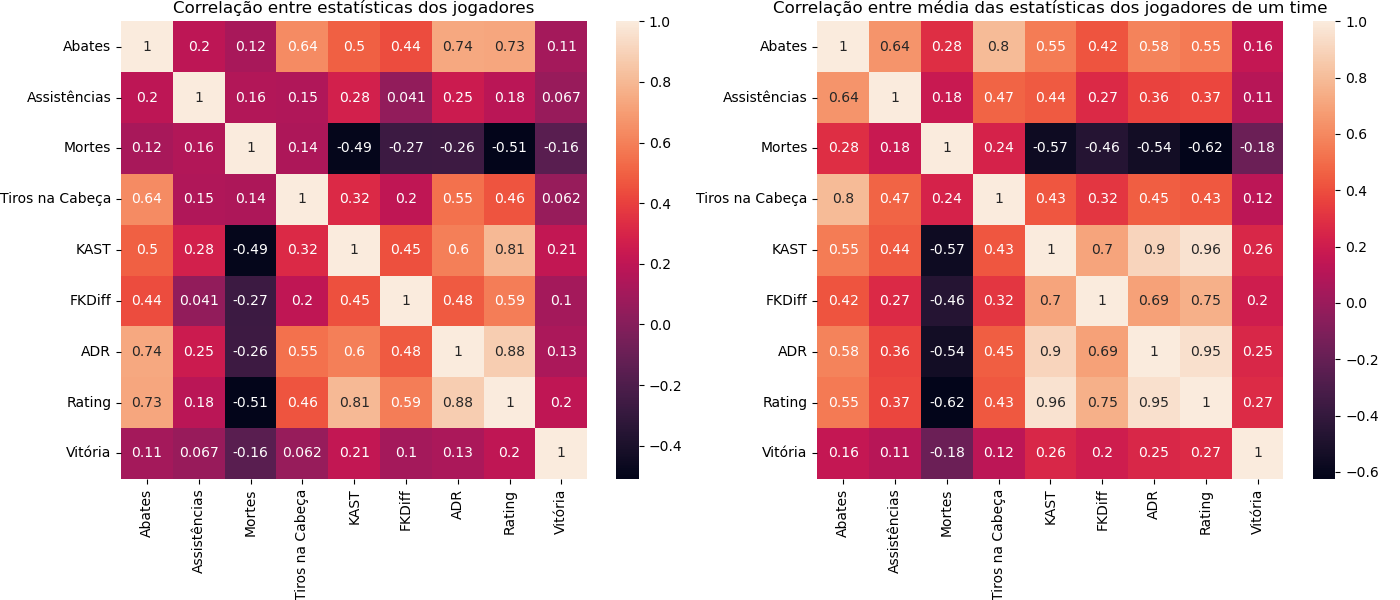
\includegraphics[width=\linewidth]{./correlacoes.png}
\end{center}

Outra maneira de descobrir quais estatísticas são as melhores para usar é medir a quantidade de entropia ganha por estatística:

\begin{center}
  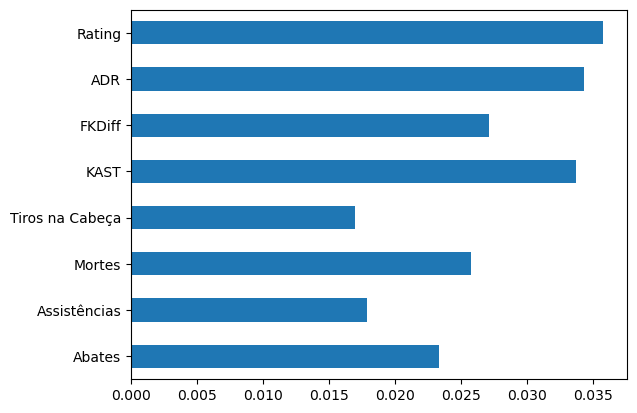
\includegraphics[width=.6\linewidth]{./information.png}
\end{center}

O que todos os dados indicam é que os campos ADR, Rating e KAST são os com maior entropia para a previsão da vitória de um time. Entretanto, vimos que os 3 campos são fortemente correlacionados, e portanto é redundante incluir os 3. Assim, iremos tentar utilizar essas features, junto de FKDiff e Mortes, para treinar modelos,e veremos a acurácia resultante.

\pagebreak

\subsection{Modelos de previsão}

Para cada dataset gerado, testamos a acurácia em 2 modelos, \textit{Random Forest Classifier} e \textit{Logistical Regression}, e medimos a acurácia ao longo de 5 tentativas (junto do desvio padrão). Para o primeiro modelo, usamos os dados que contém valores desconhecidos (NaN), enquanto para o segundo filtramos esses valores. As tabelas seguintes contém os resultados do treinamento:

\begin{table}[!h]
  \begin{center}
    \caption{\textit{Random Forest Classifier}}
    \begin{tabular}{l|rrrr}
      \toprule
      Estatísticas & Acurácia & Sensibilidade & Especificidade & Precisão \\ \midrule
      Todas                     & 66.07 & 56.23 & 74.82 & {\color{Green} 66.51} \\
      \midrule
      Deaths, FKDiff, Rating    & {\color{Green} 66.30} & 55.29 & {\color{Green} 75.74} & 66.14 \\
      Deaths, FKDiff, KAST      & 63.54 & 52.79 & 72.73 & 62.37 \\
      Deaths, FKDiff, ADR       & 64.79 & 54.76 & 73.51 & 64.28 \\
      \midrule
      Rating                    & {\color{Red} 60.17} & {\color{Red} 49.96} & {\color{Red} 68.65} & {\color{Red} 56.99} \\
      KAST                      & 63.20 & 54.85 & 70.44 & 61.69 \\
      ADR                       & 62.63 & 51.52 & 73.09 & 64.33 \\
      \midrule
      Deaths, KAST, ADR, Rating & 63.69 & {\color{Green} 56.48} & 70.17 & 62.98 \\
      Kills, Deaths, Assists    & 65.66 & 56.16 & 73.87 & 65.03 \\
      \bottomrule
    \end{tabular}
  \end{center}
\end{table}

\begin{table}[!h]
  \begin{center}
    \caption{\textit{Logistical Regression}}
    \begin{tabular}{l|rrrr}
      \toprule
      Estatísticas & Acurácia & Sensibilidade & Especificidade & Precisão \\ \midrule
      Todas                     & 66.38 & {\color{Green} 59.77} & 72.42 & 66.45 \\
      \midrule
      Deaths, FKDiff, Rating    & 65.51 & 57.96 & 72.32 & 65.40 \\
      Deaths, FKDiff, KAST      & 65.14 & 57.07 & 71.82 & 62.64 \\
      Deaths, FKDiff, ADR       & 65.97 & 57.44 & 73.26 & 64.77 \\
      \midrule
      Rating                    & {\color{Red} 61.62} & {\color{Red} 42.37} & {\color{Green} 77.17} & {\color{Red} 60.00} \\
      KAST                      & 66.51 & 58.37 & 73.49 & 65.37 \\
      ADR                       & 64.09 & 55.03 & 71.64 & 61.81 \\
      \midrule
      Deaths, KAST, ADR, Rating & 65.14 & 58.46 & 70.77 & 62.73 \\
      Kills, Deaths, Assists    & {\color{Green} 66.97} & 57.63 & 75.28 & {\color{Green} 67.46} \\
      \bottomrule
    \end{tabular}
  \end{center}
\end{table}

\section{Discussão}

Primeiramente, notamos que os resultados relativos são aproximadamente iguais para os dois métodos de classificação - isto é, não houveram casos em que um modelo conseguiu inferir coisas que o outro modelo não - mas a regressão logística apresenta resultados marginalmente melhores - maior sensibilidade, especificidade e precisão.

Em ambos os casos, o modelo que contém apenas o Rating (que deveria estar diretamente relacionado à performance) é de longe o pior, o que é surpreendente. Os valores são condizentes com a observação de que, nas partidas do dataset, o time com maior Rating médio (final, não histórico) ganhou apenas 58\% das vezes. De certa forma, conseguimos resultados melhores observando as médias históricas de cada jogador, ao invés de o Rating final na partida, mas ainda sim, não é possível extrapolar muito além disso. Além disso, notamos que incluir estatísticas de morte e de primeiro abate de cada jogador significativamente aumenta a qualidade, colocando-o no mesmo nível dos outros.

Notamos também que o KAST ou ADR por jogador são ótimas maneiras de classificar jogos, visto que apresentam resultados similares às melhores estatísticas. Isto faz sentido, pois tanto KAST quanto ADR são métricas diretamente ligadas ao quão ``participativo'' um jogador é na partida, e jogadores mais participativos tendem a impactar mais no resultado final de um jogo.

Este resultado é condizente com as taxas obtidas nos estudos feitos por \cite{navi}, que atingiu 69\% de acurácia utilizando redes neurais com XGBoost, e \cite{glicko2} que atingiu 60\% de acerto utilizando o algoritmo de Glicko2 rating.

\section{Conclusão}

Para diminuir a complexidade, o modelo escolhido faz diversas simplificações que dificultam a previsão. Primeiramente, assumimos que todos os jogos tem impacto igual nas estatísticas passadas; isto é, se um jogador performou muito bem em uma partida contra um oponente difícil, e performou mal numa partida contra um oponente fácil, não é feita nenhuma distinção nessas estatísticas na hora de pre-processar os dados. Para remediar isso, poderíamos implementar algum tipo de sistema de rating, que utiliza a força do oponente (e a própria força) para balancear os resultados. Da mesma forma, se um jogador joga apenas contra times fracos, suas estatísticas são menos relevantes do que um jogador que consistentemente joga contra os melhores times.

Além disso, ignoramos completamente o aspecto da economia do jogo, que é crucial para determinar a vitória. Decisões econômicas - como decidir entre comprar armas ruins ou guardar dinheiro para o próximo round - afetam diretamente a chance de vitória em uma partida (já que uma decisão ruim pode afetar múltiplos rounds), e times bons consistentemente farão boas decisões. De alguma forma, isso estará eventualmente ligado às estatísticas, já que times que tomam melhores decisões econômicas tendem a ter uma taxa maior de sucesso, mas estamos ignorando completamente as estatísticas no \textbf{economy.csv}.

Também ignoramos os mapas jogados, e é extremamente comum ver jogadores de alto nível performarem melhor em mapas específicos. Para remediar isso, poderíamos tentar calcular as estatísticas específicas associadas a cada mapa, mas isso também diminuiria os resultados de partidas num geral, e aumentaria a complexidade do modelo.

Por fim, é importante ressaltar que grande parte da graça de (e)sportes é que os resultados são imprevisíveis. Intuitivamente, sabemos que a assunção de que um time com estatísticas melhores sempre vencerá não é sempre verdadeira, e inúmeras vezes vemos resultados inesperados acontecendo, o que torna a previsão de jogos ainda mais difícil. Fatores como cansaço, humor, pressão, bem estar de cada jogador e várias outras métricas influenciam diretamente no resultado do jogo, e infelizmente nunca teremos esses dados. Ainda sim, conseguimos atingir resultados significativamente melhores do que 50\% (chute aleatório) o que significa que essa assunção vale para a maioria dos casos.

\def\UrlBreaks{\do\/\do-}
\bibliographystyle{sbc}
\bibliography{sbc-template}

\end{document}
